%
% - - - - - - - Supplemental material from body of paper, Jan. 14 2020.
%

\section{Supplemental Material}
\label{sec:Supp}

\subsection{Additional comparisons between PDF sets}
\label{sec:Supp-PDFbands}

\begin{figure}[b]
\hspace*{-1.5cm}
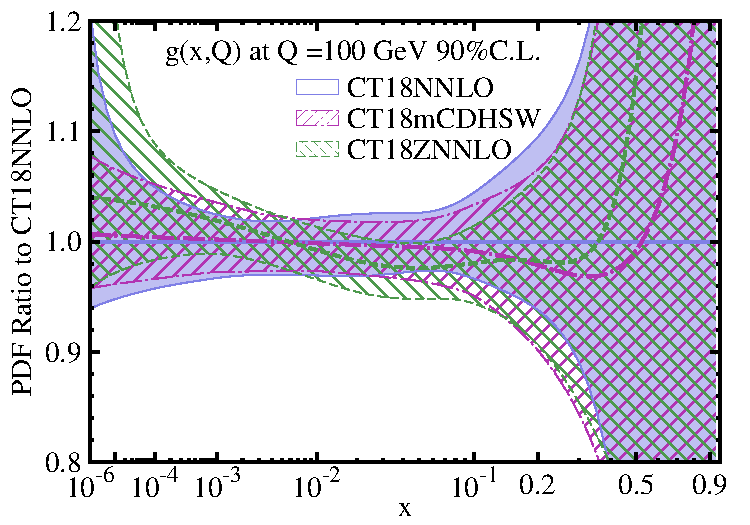
\includegraphics[width=0.49\textwidth]{./fig/SuppMat/pdfs_CT18NNLO_CT18mCDHSW_CT18ZNNLO_100GeV_A90CL__00___glu__pdfr_cus-lin_ect.pdf}
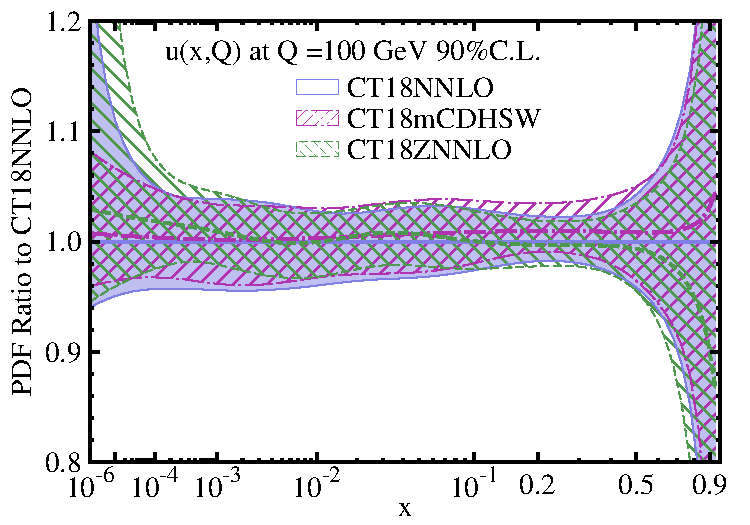
\includegraphics[width=0.49\textwidth]{./fig/SuppMat/pdfs_CT18NNLO_CT18mCDHSW_CT18ZNNLO_100GeV_A90CL__01___uqk__pdfr_cus-lin_ect.pdf}\\
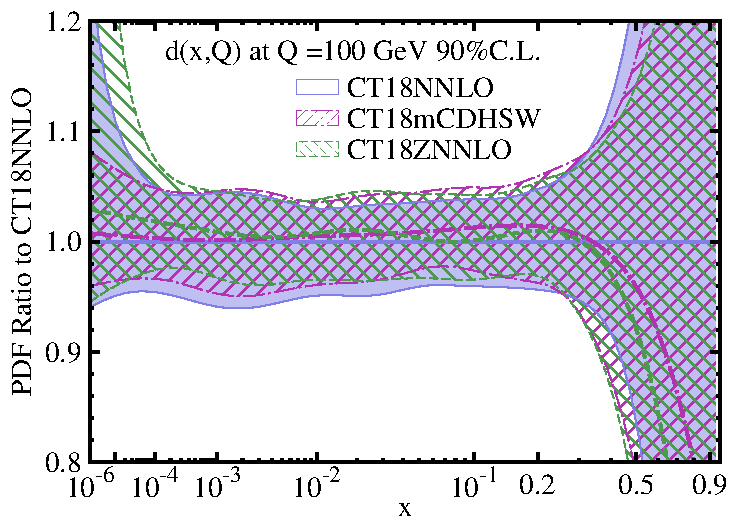
\includegraphics[width=0.49\textwidth]{./fig/SuppMat/pdfs_CT18NNLO_CT18mCDHSW_CT18ZNNLO_100GeV_A90CL__02___dqk__pdfr_cus-lin_ect.pdf}
\caption{Effect of eliminating CDHSW data (Exp.~IDs=108, 109) from the CT18 fit. CT18mCDHSW denotes the fit after removing the CDHSW data sets. The result of CT18Z fit is also shown for comparison. 
\label{fig:cdhsw}}
\end{figure}

%
\begin{figure}
	\begin{tabular}{cc}
		\subfloat[NNLO $g(x,Q = 100\,\mathrm{GeV})$, CT18(Z) vs.~CT18A]{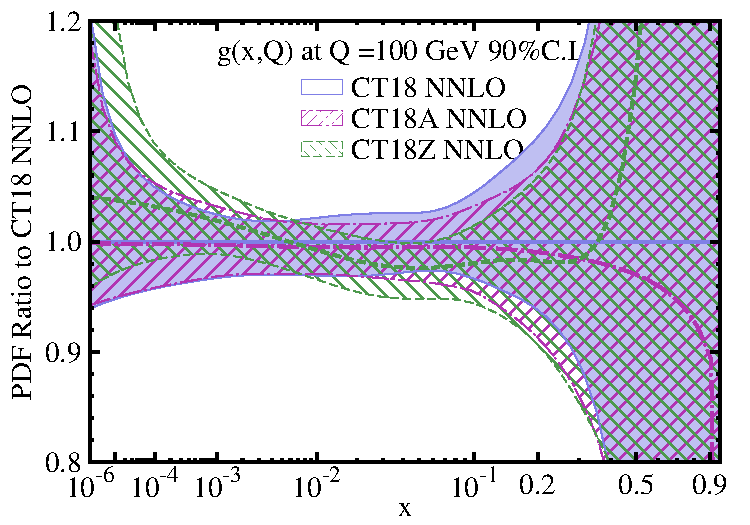
\includegraphics[width=0.49\textwidth]{fig/SuppMat/g_AZ_ect.pdf}} &
		\subfloat[NNLO $g(x,Q = 100\,\mathrm{GeV})$, CT18(Z) vs.~CT18X]{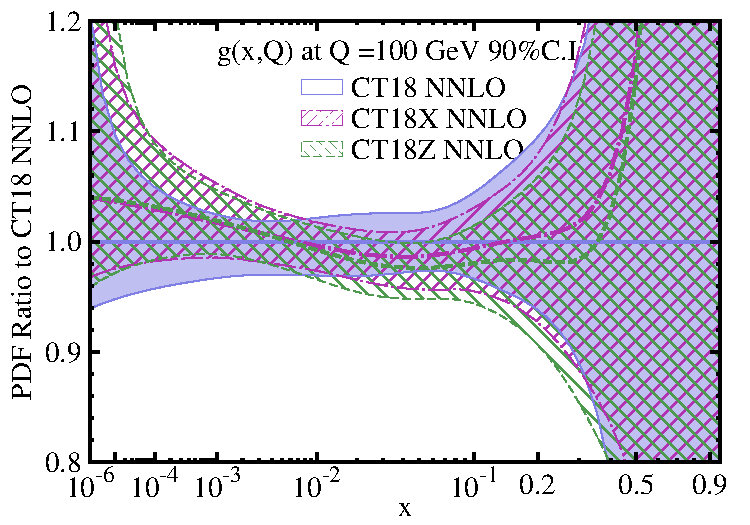
\includegraphics[width=0.49\textwidth]{fig/SuppMat/g_XZ_ect.pdf}}\\
		\subfloat[NLO  $g(x,Q = 100\,\mathrm{GeV})$, CT18(Z) vs.~CT18A]{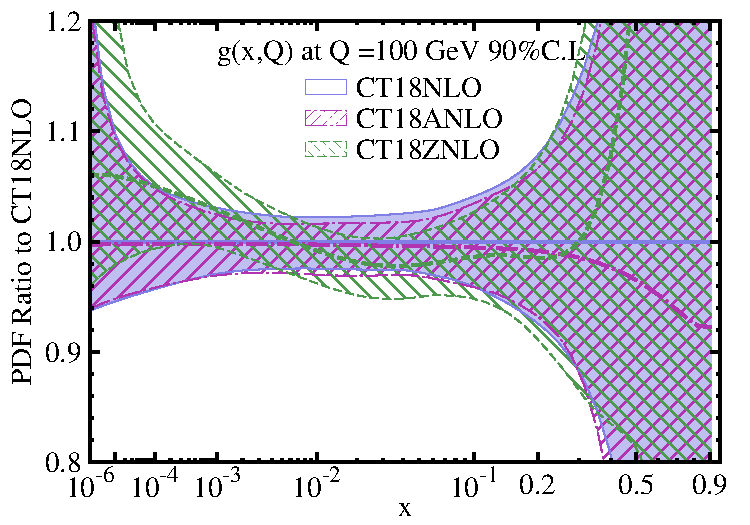
\includegraphics[width=0.49\textwidth]{fig/SuppMat/g_AZ_NLO_ect.pdf}} &
		\subfloat[NLO  $g(x,Q = 100\,\mathrm{GeV})$, CT18(Z) vs.~CT18X]{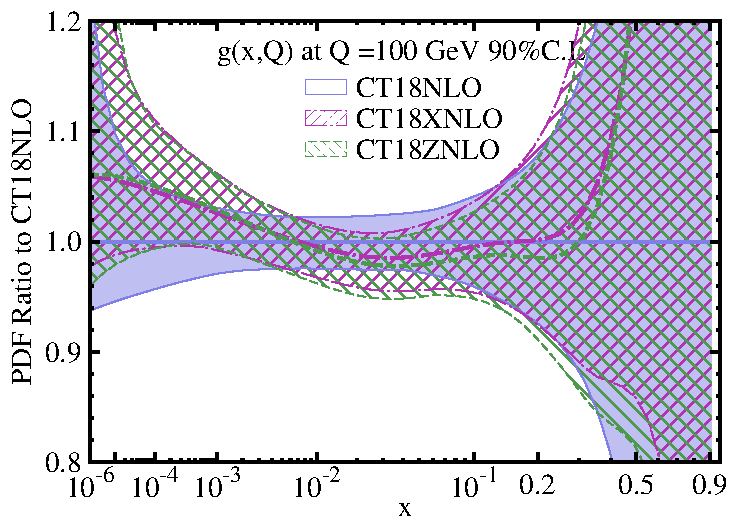
\includegraphics[width=0.49\textwidth]{fig/SuppMat/g_XZ_NLO_ect.pdf}}
	\end{tabular}
	\caption{
		Gluon PDF ratios for the CT18Z and CT18A/X alternative fits, evaluated with respect to the primary, CT18 result. In
		the left panels [(a) and (c)], we compare CT18(Z) against CT18A, whereas the right panels [(b) and (d)] overlay CT18(Z) with CT18X. In addition,
		we examine differences for NNLO and NLO fits; the upper panels [(a) and (b)] are NNLO, and
		the lower panels [(c) and (d)] are NLO.
	}
\label{fig:glu_AXZ}
\end{figure}

%
\begin{figure}
	\begin{tabular}{cc}
		\subfloat[NNLO $d(x,Q = 100\,\mathrm{GeV})$, CT18(Z) vs.~CT18A]{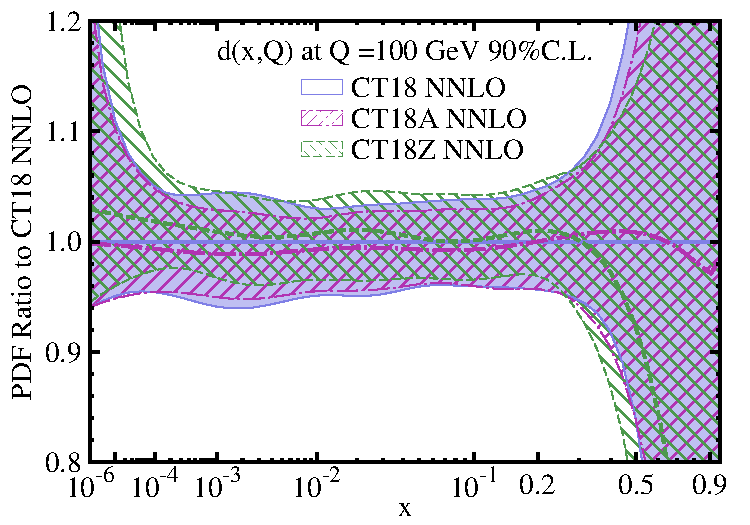
\includegraphics[width=0.49\textwidth]{fig/SuppMat/d_AZ_ect.pdf}} &
		\subfloat[NNLO $d(x,Q = 100\,\mathrm{GeV})$, CT18(Z) vs.~CT18X]{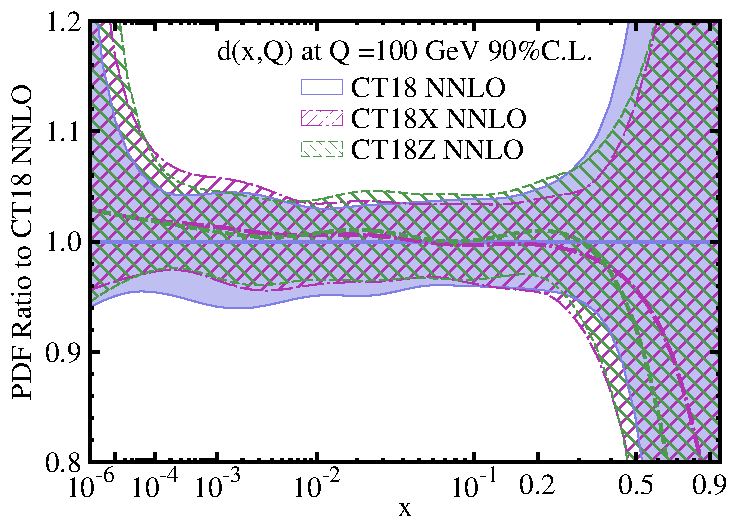
\includegraphics[width=0.49\textwidth]{fig/SuppMat/d_XZ_ect.pdf}}\\
		\subfloat[NLO  $d(x,Q = 100\,\mathrm{GeV})$, CT18(Z) vs.~CT18A]{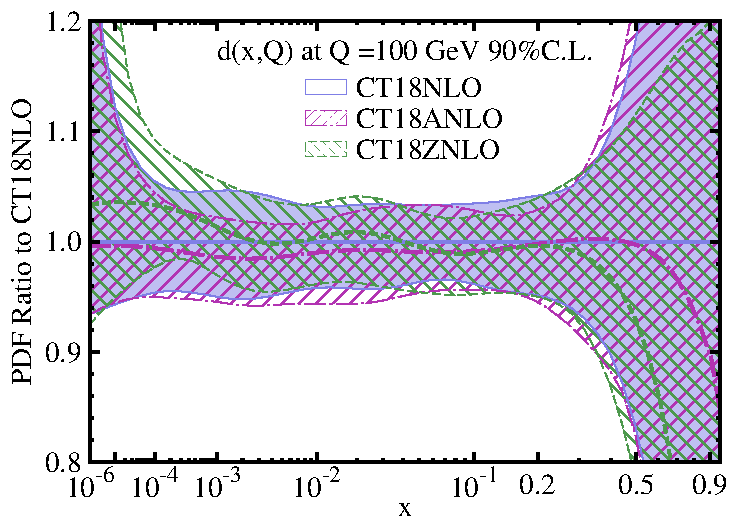
\includegraphics[width=0.49\textwidth]{fig/SuppMat/d_AZ_NLO_ect.pdf}} &
		\subfloat[NLO  $d(x,Q = 100\,\mathrm{GeV})$, CT18(Z) vs.~CT18X]{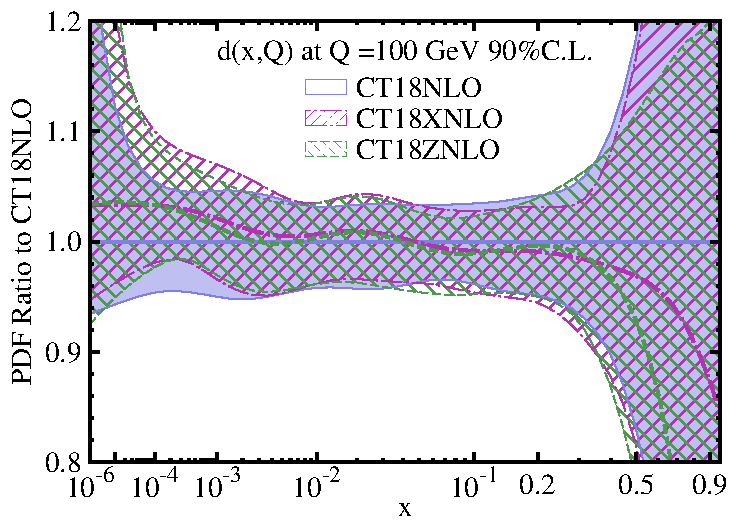
\includegraphics[width=0.49\textwidth]{fig/SuppMat/d_XZ_NLO_ect.pdf}}
	\end{tabular}
	\caption{
		A comparison of the $d$-quark PDF ratios with respect to CT18 for the CT18(Z) PDFs vs.~the CT18A/X alternative fits.
		The plots here are analogous to those shown for the gluon in Fig.~\ref{fig:glu_AXZ}.
	}
\label{fig:d_AXZ}
\end{figure}
%

\begin{figure}
	\begin{tabular}{cc}
		\subfloat[NNLO $\bar{u}(x,Q = 100\,\mathrm{GeV})$, CT18(Z) vs.~CT18A]{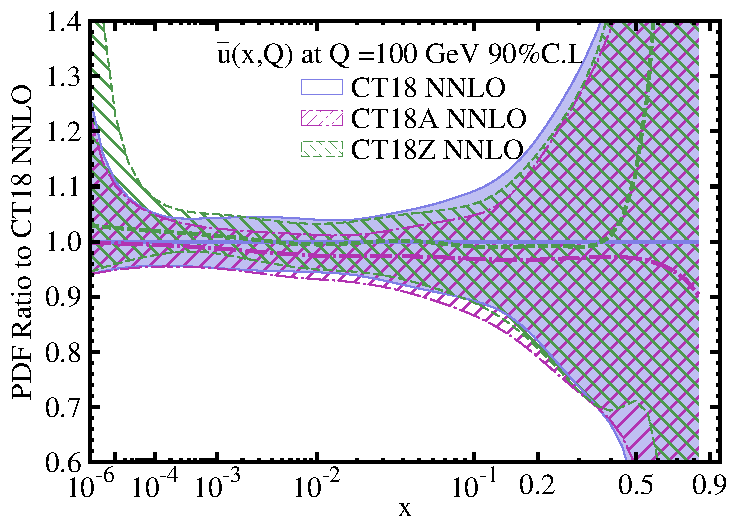
\includegraphics[width=0.49\textwidth]{fig/SuppMat/ubar_AZ_ect.pdf}} &
		\subfloat[NNLO $\bar{u}(x,Q = 100\,\mathrm{GeV})$, CT18(Z) vs.~CT18X]{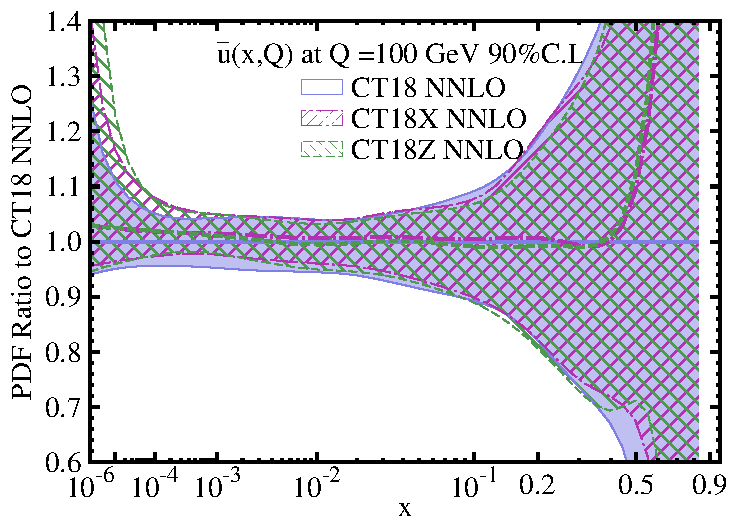
\includegraphics[width=0.49\textwidth]{fig/SuppMat/ubar_XZ_ect.pdf}}\\
	\end{tabular}
	\caption{
		As with Fig.~\ref{fig:d_AXZ}, we explore the $\bar{u}$-antiquark PDF ratios at NNLO,
		comparing CT18(Z) with CT18A NNLO in panel (a), and with CT18X in panel (b).
	}
\label{fig:ubar_AXZ}
\end{figure}

\begin{figure}[tb]
	\begin{tabular}{cc}
		\subfloat[NNLO $s(x,Q = 100\,\mathrm{GeV})$, CT18(Z) vs.~CT18A]{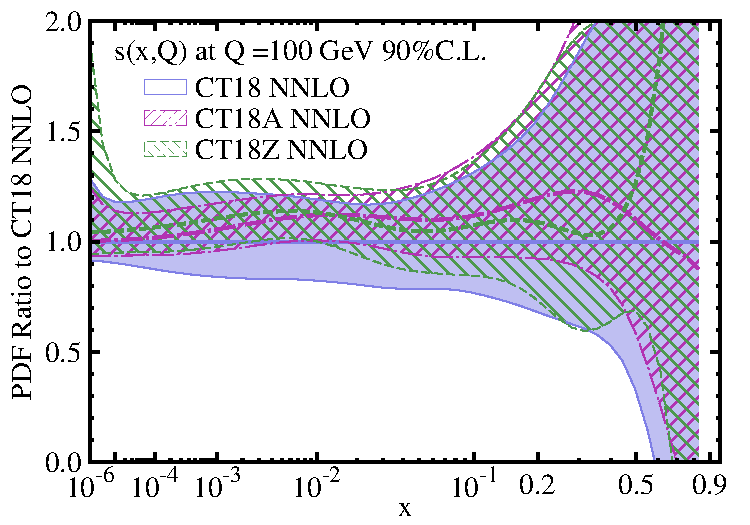
\includegraphics[width=0.49\textwidth]{fig/SuppMat/s_AZ_ect.pdf}} &
		\subfloat[NNLO $s(x,Q = 100\,\mathrm{GeV})$, CT18(Z) vs.~CT18X]{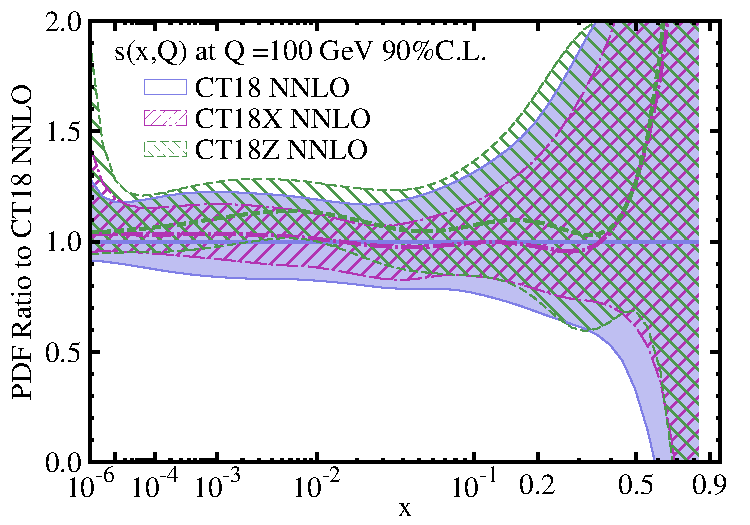
\includegraphics[width=0.49\textwidth]{fig/SuppMat/s_XZ_ect.pdf}}\\
	\end{tabular}
	\caption{
		Like Fig.~\ref{fig:ubar_AXZ}, but now comparing alternative distributions for the nucleon strangeness, $s(x,Q)$.
	}
\label{fig:s_AXZ}
\end{figure}

\begin{figure}[tb]
	\begin{tabular}{cc}
		\subfloat[NNLO $R_s(x,Q = 100\,\mathrm{GeV})$, CT18(Z) vs.~CT18A]{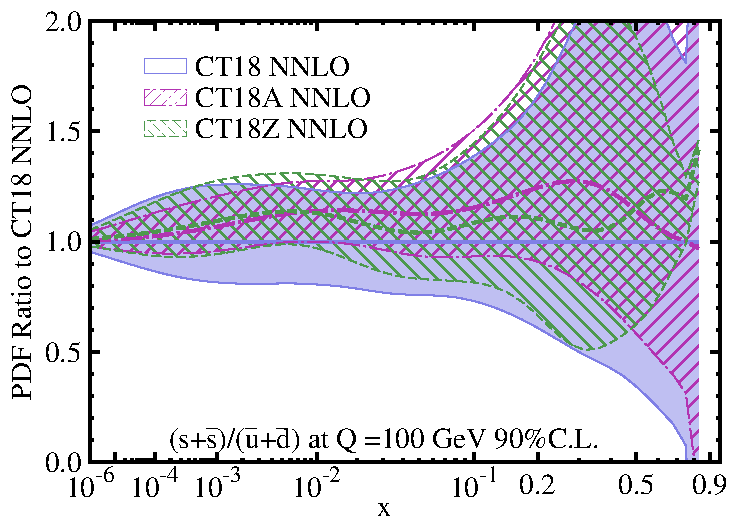
\includegraphics[width=0.49\textwidth]{fig/SuppMat/Rs_AZ_ect.pdf}} &
		\subfloat[NNLO $R_s(x,Q = 100\,\mathrm{GeV})$, CT18(Z) vs.~CT18X]{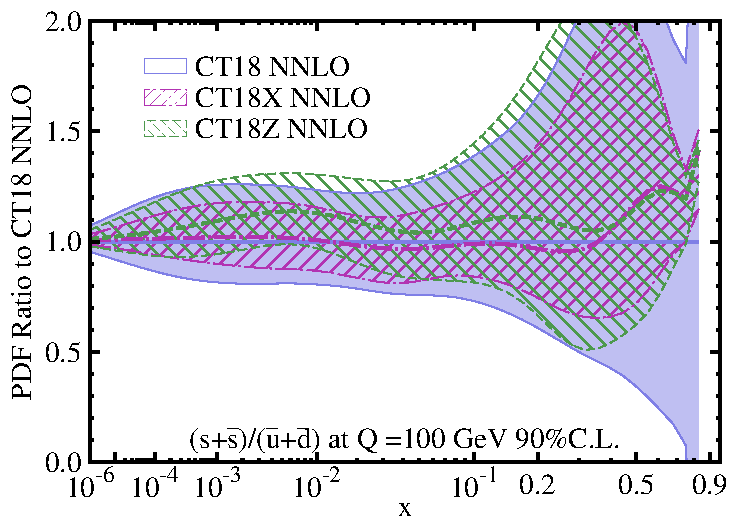
\includegraphics[width=0.49\textwidth]{fig/SuppMat/Rs_XZ_ect.pdf}}\\
	\end{tabular}
	\caption{
		The strange suppression factor, $R_s\! \equiv\! (s+\bar s) / (\bar u + \bar d)$, for the CT18(Z) and CT18A/X NNLO alternative fits, evaluated with respect to the primary,
		CT18 NNLO result.
	}
\label{fig:Rs_AXZ}
\end{figure}

\begin{figure}[p]
\center
  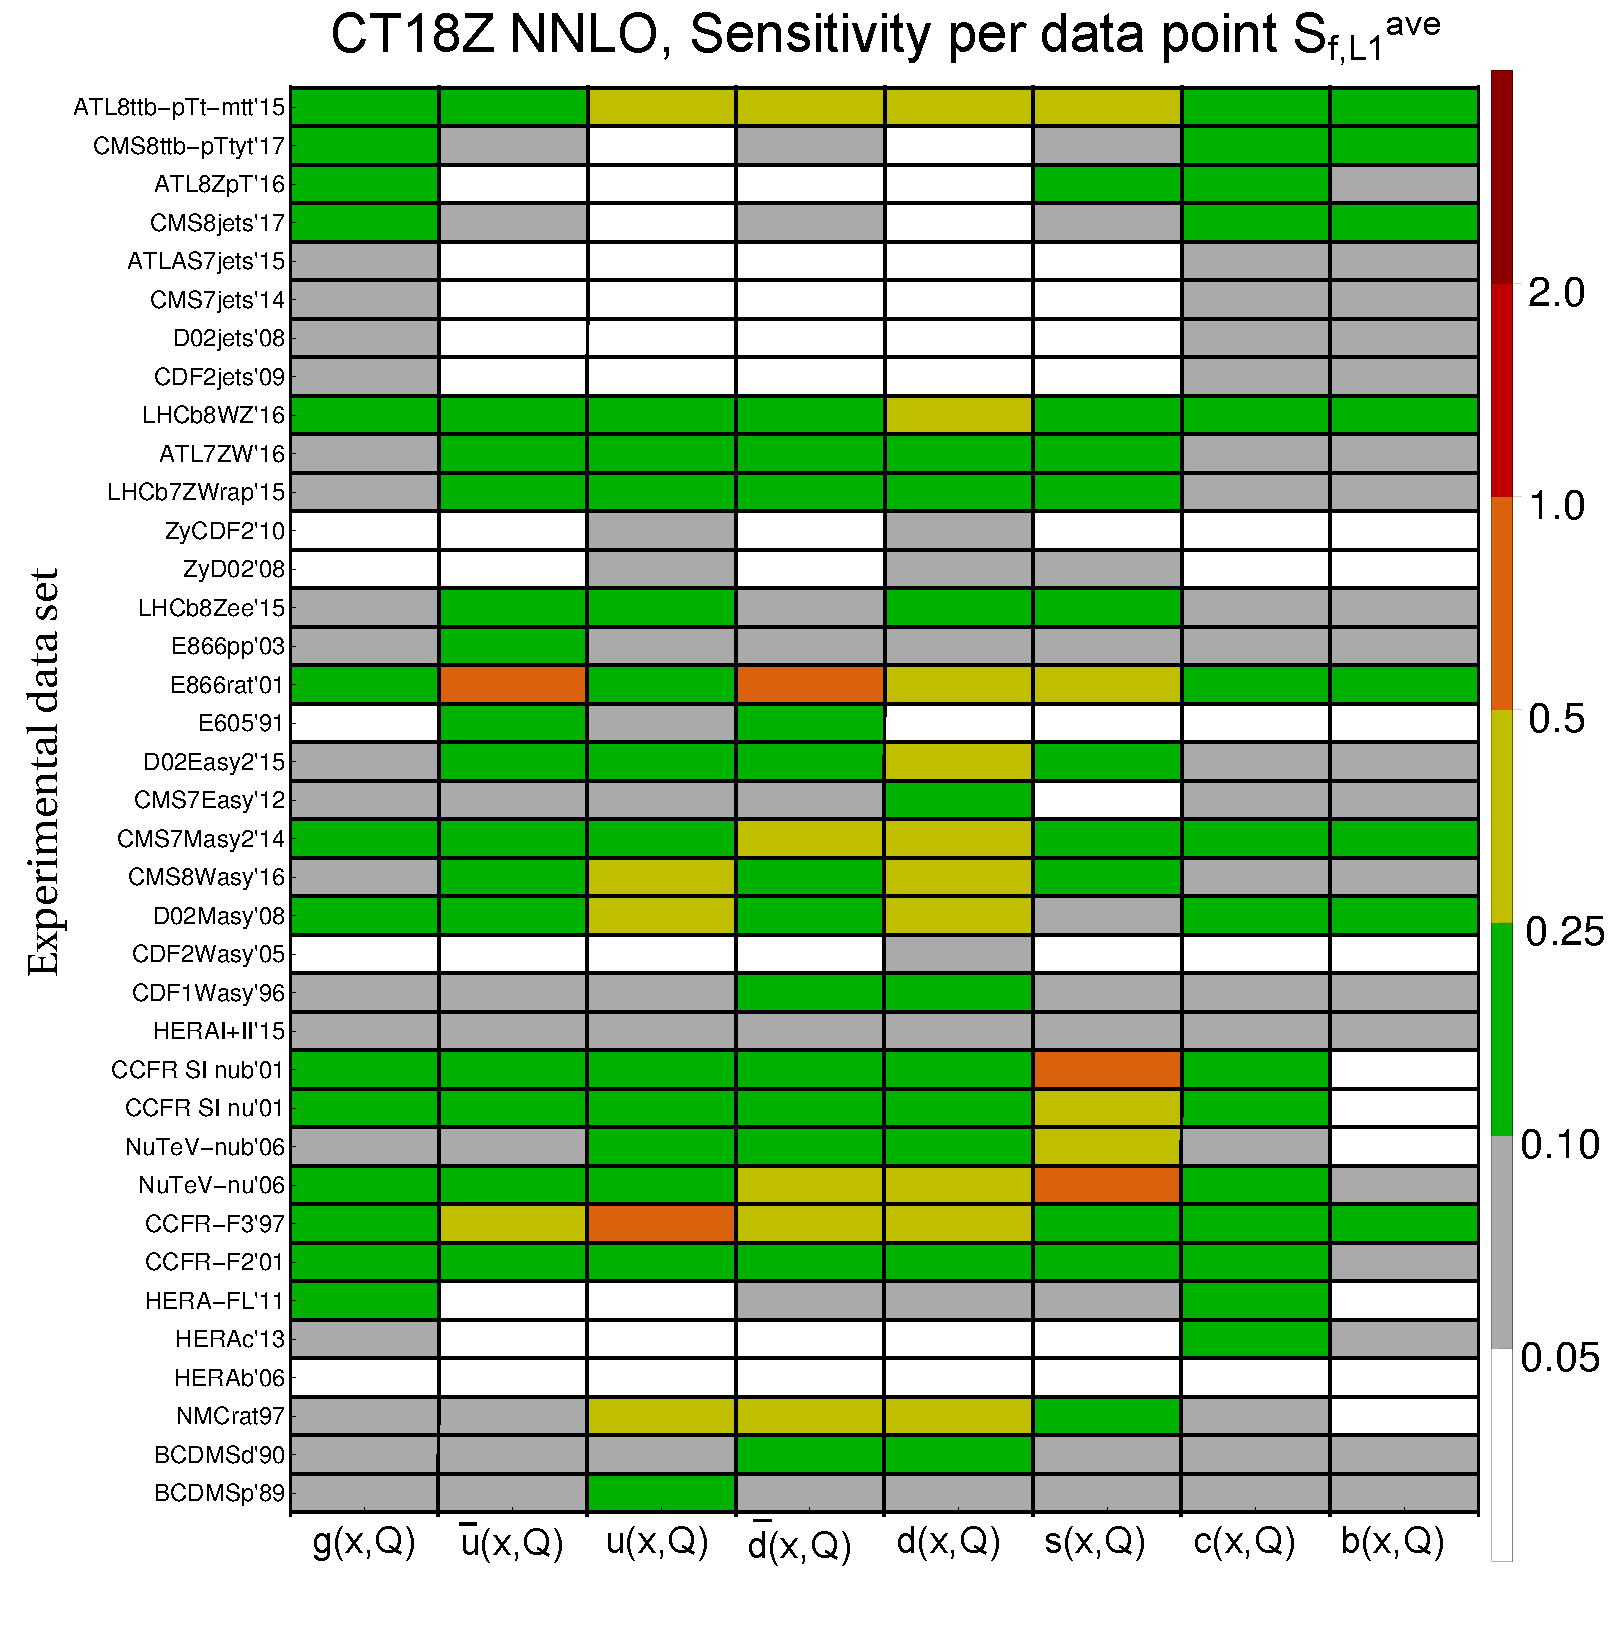
\includegraphics[width=0.59 \textwidth]{./fig/SuppMat/ave_S_bycolor_ct18znn.pdf}\\ 
  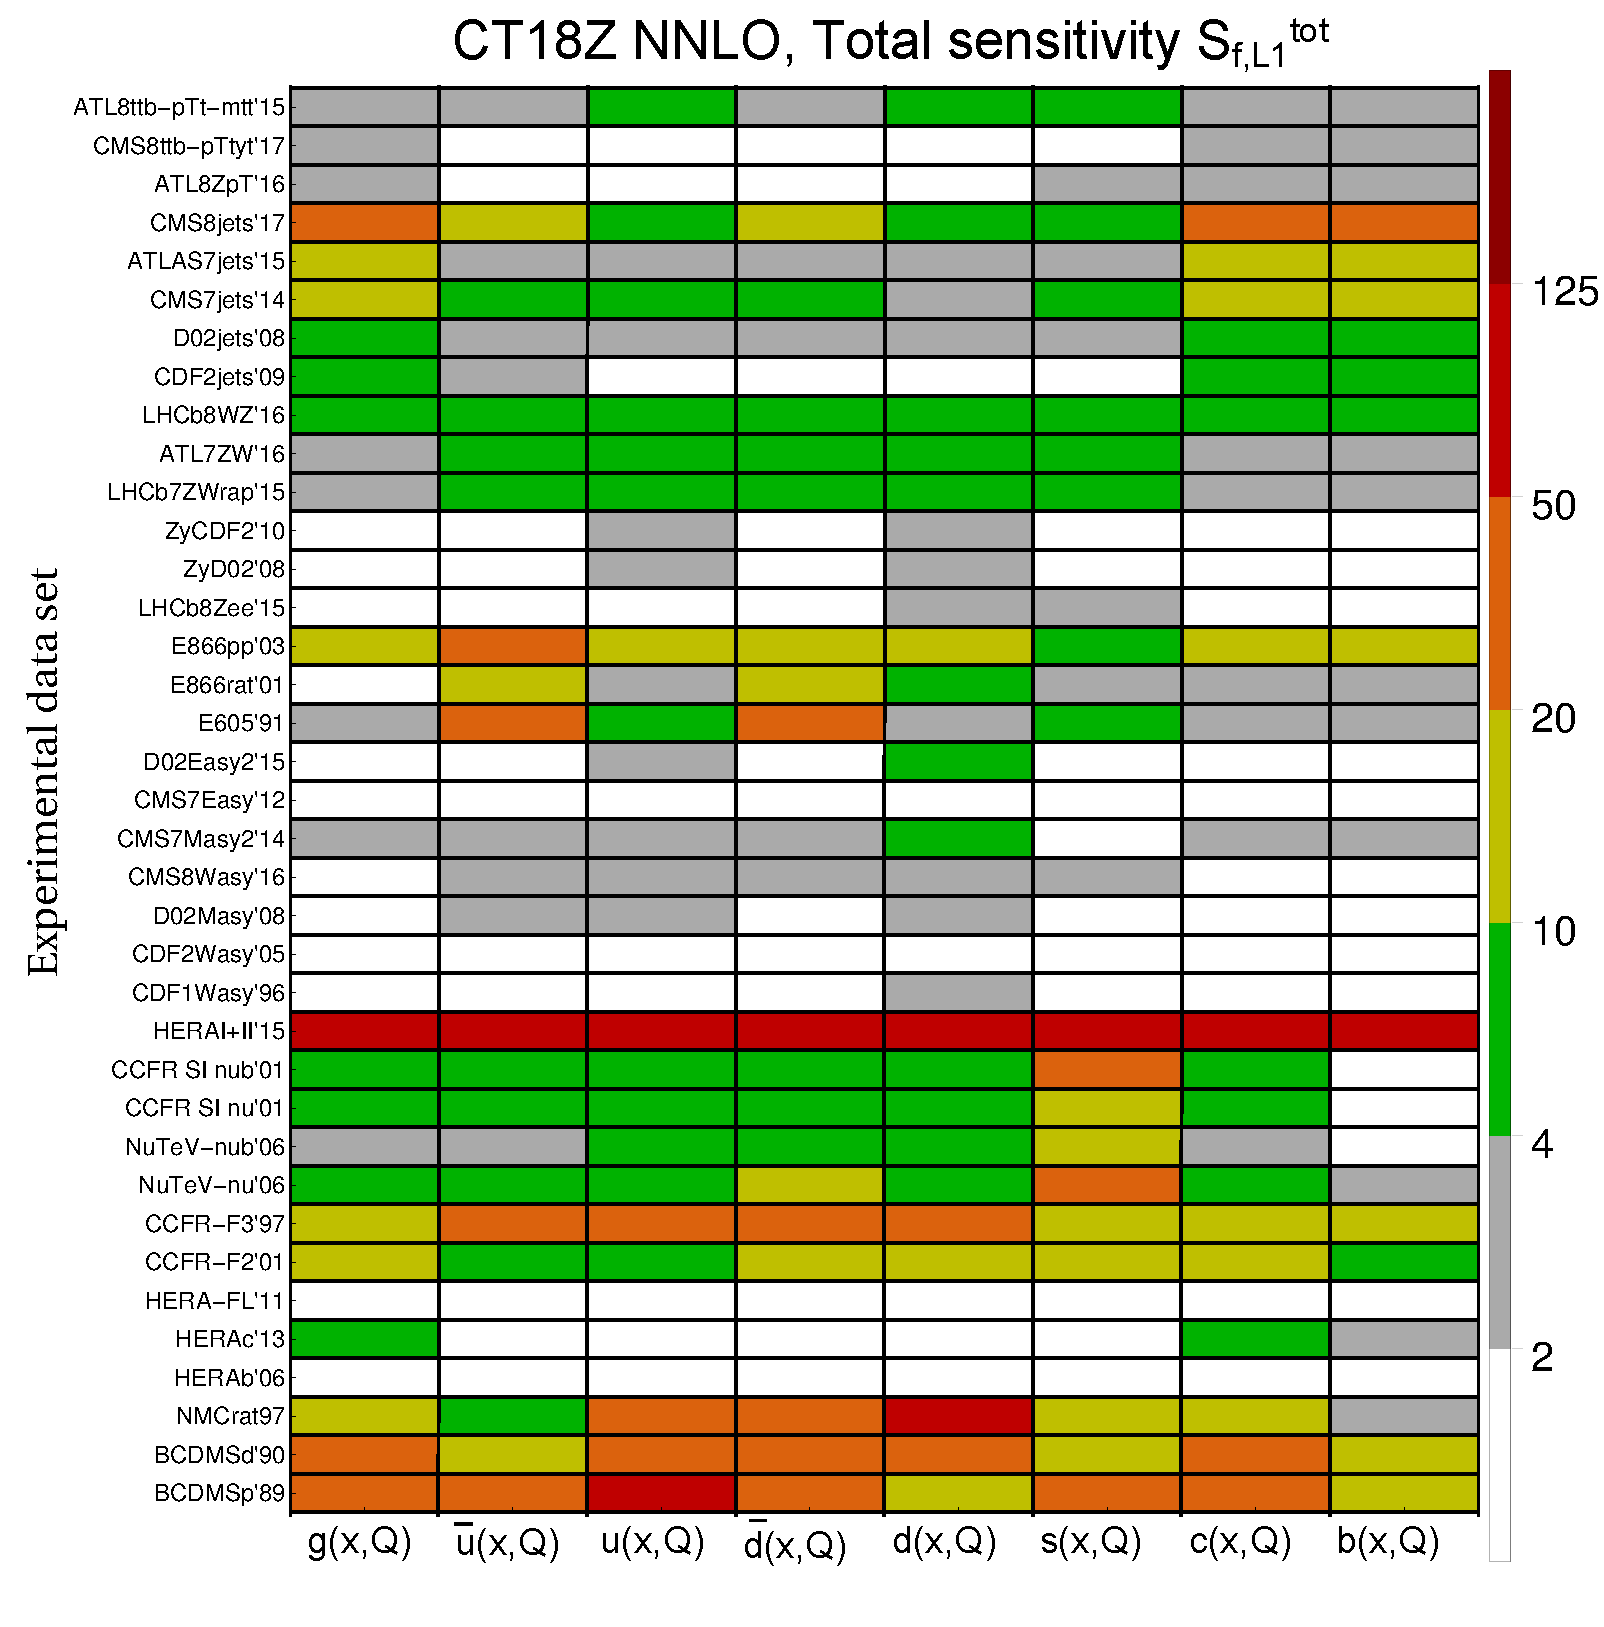
\includegraphics[width=0.59\textwidth]{./fig/SuppMat/total_S_bycolor_ct18znn.pdf}
        	\caption{$L_1$ sensitivities of experimental data
                  sets to PDF flavors in the CT18Z NNLO analysis,
                  computed according to the methodology in
               Ref.~\cite{Wang:2018heo}. The color of the cells
                  in the upper (lower) inset, 
                  chosen according to the palettes on the right,
                  indicates the point-average
                  (cumulative) sensitivity of the experimental set
                  on the vertical axis to the PDF flavor
                  on the horizontal axis. 
		\label{fig:CT18Zquilts}}
\end{figure}

\clearpage

\subsection{Additional histograms}
\label{sec:Supp-hist}

The residuals and nuisance parameters for Exp.~ID=249 are shown in
Fig.~\ref{fig:resnui249}. Both are reasonably compatible with the
normal distribution with mean 0 and standard deviation 1. 
%
\begin{figure}[htbp]
	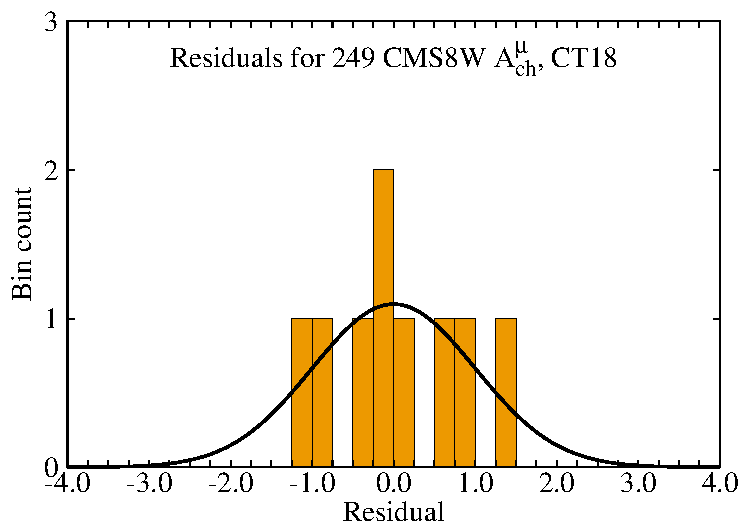
\includegraphics[width=0.49\textwidth]{./fig/SuppMat/res_his_CT18-249_4_ect.pdf}
	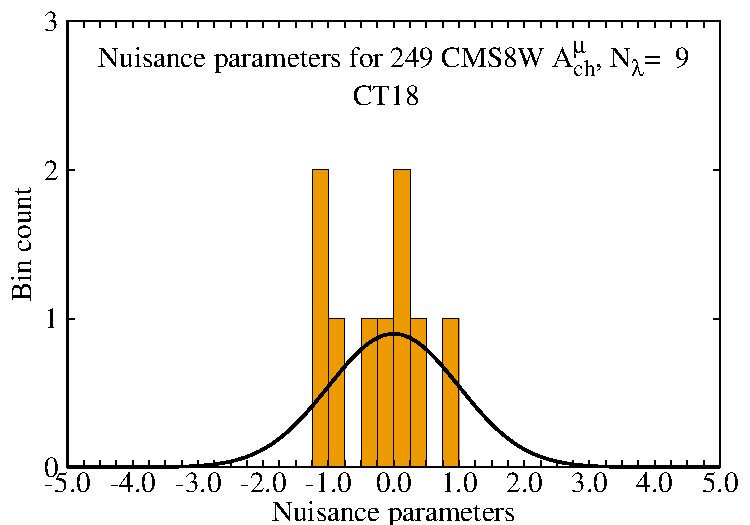
\includegraphics[width=0.49\textwidth]{./fig/SuppMat/rk_his_CT18-249__4_ect.pdf}
	\caption{Distribution of residuals (left) and nuisance parameters (right) for the CMS 8 TeV $W$-lepton charge asymmetry data (Exp.~ID=249).
	}
\label{fig:resnui249}
\end{figure}


%
The overall quality of the fit to the combined LHC jet data is 
demonstrated by the distributions of residuals and the fitted 
values of nuisance parameters, shown in
Figs.~\ref{fig:res_rk_2} and \ref{fig:res_rk_4}.
%
\begin{figure}[htbp]
	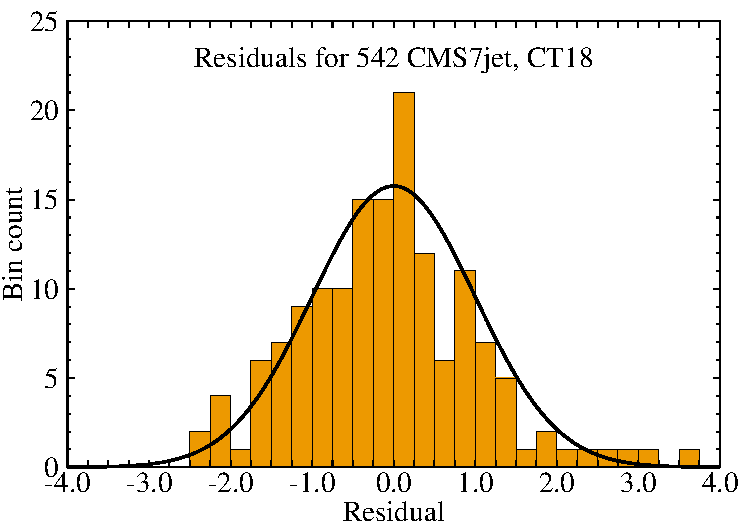
\includegraphics[width=0.32\textwidth]{./fig/SuppMat/res_his_CT18-542_4_ect.pdf}
	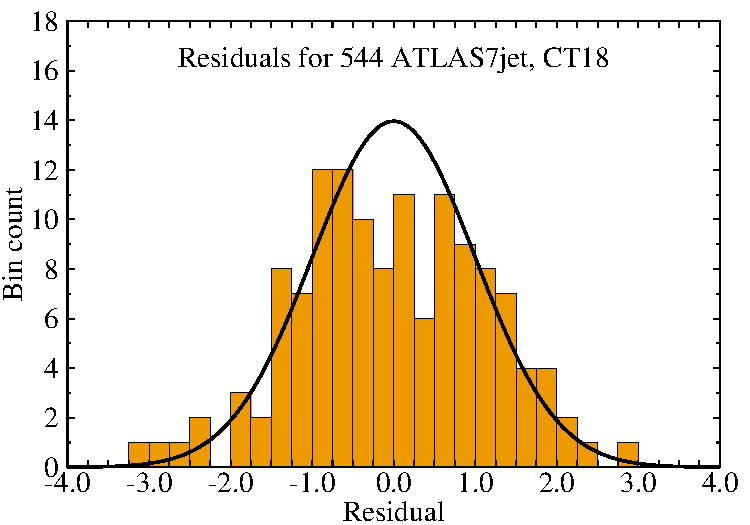
\includegraphics[width=0.32\textwidth]{./fig/SuppMat/res_his_CT18-544_4_ect.pdf}
	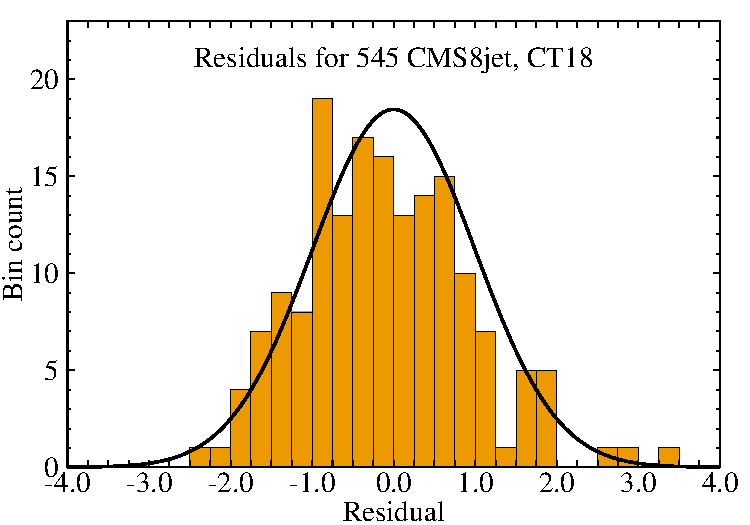
\includegraphics[width=0.32\textwidth]{./fig/SuppMat/res_his_CT18-545_4_ect.pdf}
	\caption{We plot histograms giving the distribution of shifted residuals, $r_i$ of Eq.~(\ref{eq:res-cov}), for each of the newly-included
	LHC jet experiments: the CMS 7 TeV data (Exp.~ID=542, left), ATLAS 7 TeV (Exp.~ID=544, center), and the CMS 8 TeV jet data (Exp.~ID=545, right).
		\label{fig:res_rk_2}}
\end{figure}

\begin{figure}[htbp]
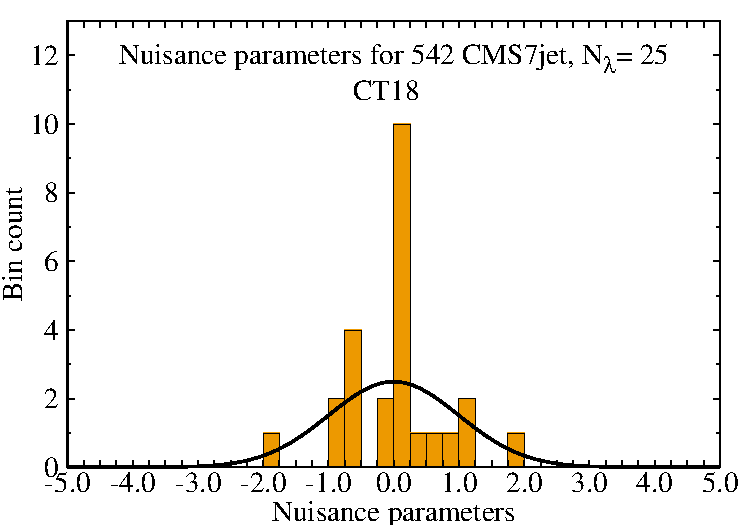
\includegraphics[width=0.32\textwidth]{./fig/SuppMat/rk_his_CT18-542__4_ect.pdf}
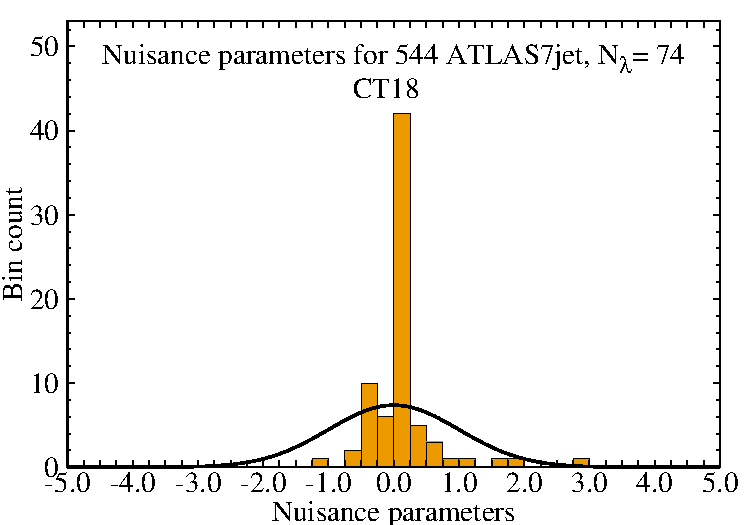
\includegraphics[width=0.32\textwidth]{./fig/SuppMat/rk_his_CT18-544__4_ect.pdf}
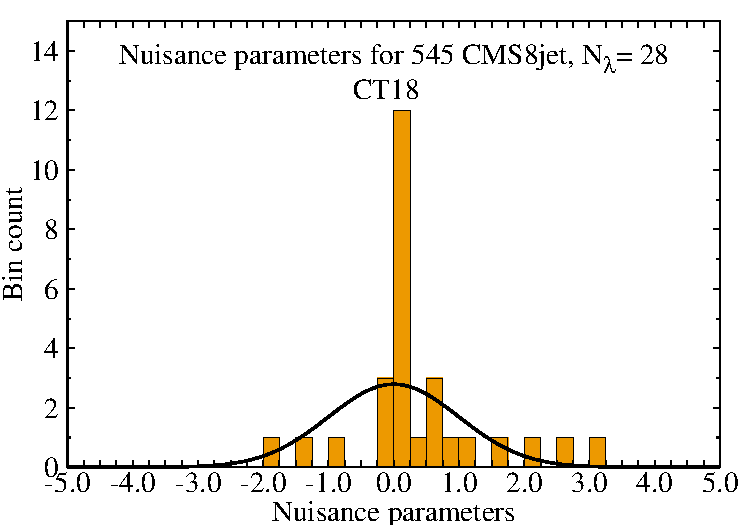
\includegraphics[width=0.32\textwidth]{./fig/SuppMat/rk_his_CT18-545__4_ect.pdf}
\caption{Like Fig.~\ref{fig:res_rk_2}, but now for the distribution of nuisance parameters obtained for the CMS 7 TeV data (Exp.~ID=542, left), ATLAS 7 TeV
	(Exp.~ID=544, center), and the CMS 8 TeV jet data (Exp.~ID=545, right).
}
\label{fig:res_rk_4}
\end{figure}


\begin{figure}[htbp]
	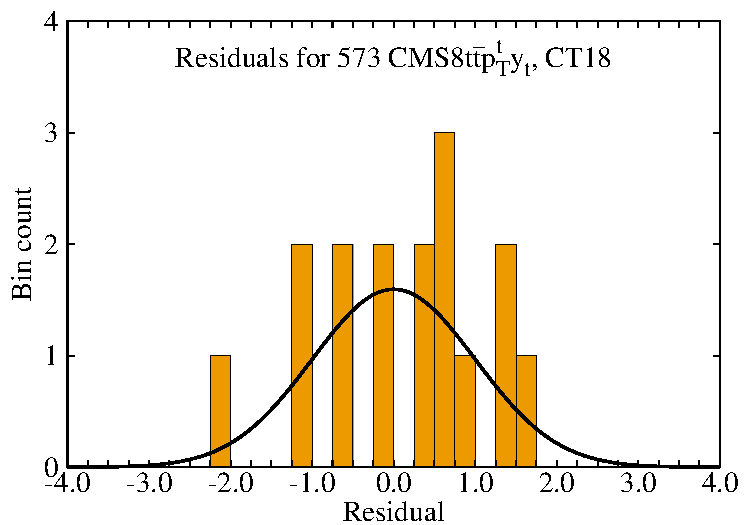
\includegraphics[width=0.4\textwidth]{./fig/SuppMat/res_his_CT18-573_4_ect.pdf}
	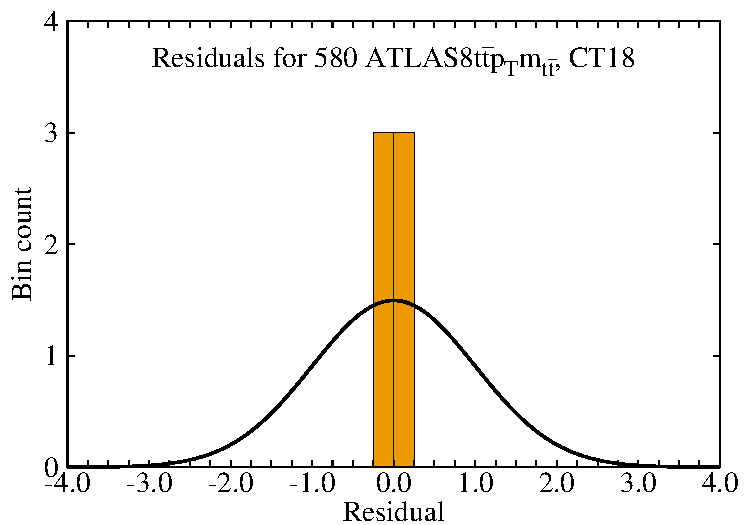
\includegraphics[width=0.4\textwidth]{./fig/SuppMat/res_his_CT18-580_4_ect.pdf}
	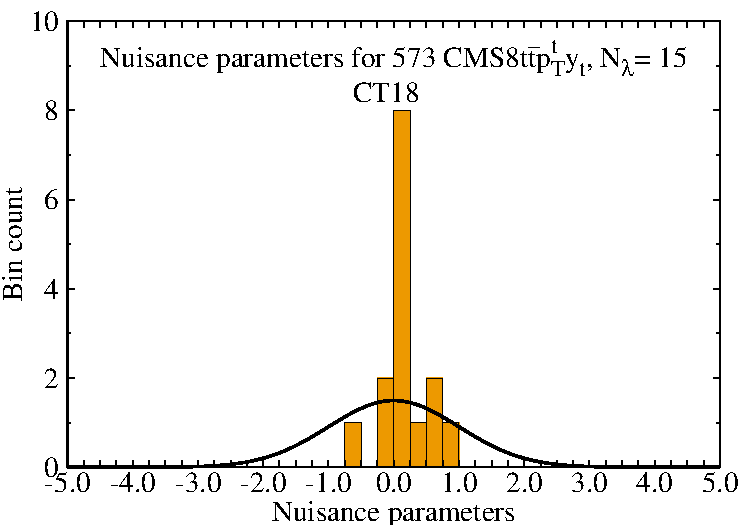
\includegraphics[width=0.4\textwidth]{./fig/SuppMat/rk_his_CT18-573__4_ect.pdf}
	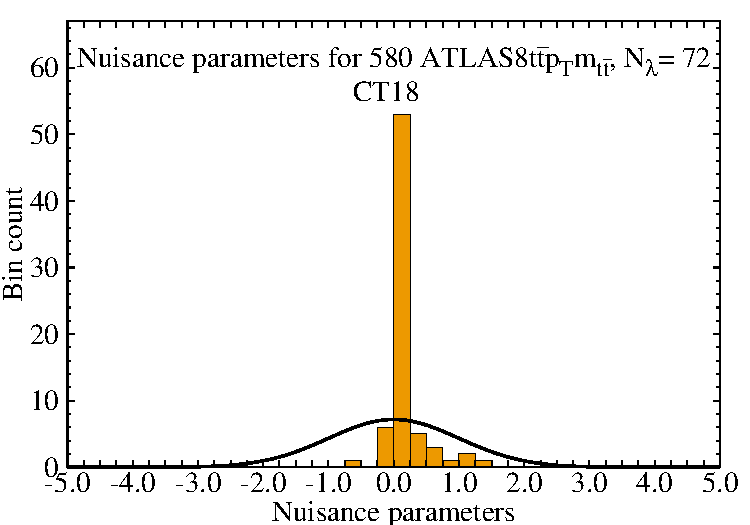
\includegraphics[width=0.4\textwidth]{./fig/SuppMat/rk_his_CT18-580__4_ect.pdf}
	\caption{Distribution of residuals (upper panels) and nuisance parameters (lower panels)
	for the CMS (left panels, Exp.~ID=573) and ATLAS (right panels, Exp.~ID=580) 2D top
	quark pair data.
	\label{fig:res_rk_7}}
\end{figure}
